% =====================================================================
% Supplementary Information for paper06_assessment_separation_v77
% =====================================================================
\documentclass[preprint,11pt,authoryear]{elsarticle}
\usepackage{amsmath,amssymb,amsthm}
\usepackage{booktabs}
\usepackage{array}
\usepackage{tabularx}
\usepackage{graphicx}
\graphicspath{{./}{figs/}{paper06_assessment_separation_v77_src/figs/}}
\usepackage{enumitem}
\usepackage[colorlinks=true,urlcolor=blue,linkcolor=blue,citecolor=blue]{hyperref}
\usepackage{xr}
\externaldocument[main-]{paper06_assessment_separation_v77}
\emergencystretch=3em
\setlength{\tolerance}{2000}

\renewcommand{\thesection}{S\arabic{section}}
\renewcommand{\thetable}{S\arabic{table}}
\renewcommand{\thefigure}{S\arabic{figure}}
\renewcommand{\theequation}{S\arabic{equation}}
\newtheorem{theorem}{Theorem}
\renewcommand{\thetheorem}{S\arabic{theorem}}
\newtheorem{lemma}{Lemma}
\renewcommand{\thelemma}{S\arabic{lemma}}
\newtheorem{proposition}{Proposition}
\renewcommand{\theproposition}{S\arabic{proposition}}
\theoremstyle{remark}
\newtheorem{remark}{Remark}
\renewcommand{\theremark}{S\arabic{remark}}

\newcommand{\Etyp}{E_{\mathrm{typ}}}
\newcommand{\Eend}{E_{\mathrm{end}}}
\newcommand{\Ephys}{E_{\mathrm{tube,phys}}}
\newcommand{\Vtyp}{\mathcal{V}_{\mathrm{typ}}}
\newcommand{\Vweak}{\mathcal{V}_{\mathrm{weak}}}
\newcommand{\Vphys}{\mathcal{V}_{\mathrm{phys}}}
\newcommand{\Vend}{\mathcal{V}_{\mathrm{end}}}
\newcommand{\Wp}{W_+}
\newcommand{\FP}{\mathrm{FP}_{\mathrm{agg}}}
\newcommand{\Tube}{\mathrm{Tube}}
\newcommand{\Succ}{\mathrm{Succ}}
\newcommand{\End}{\mathrm{End}}
\newcommand{\conv}{\operatorname{conv}}
\newcommand{\Rp}{\mathbb{R}^n_+}
\newcommand{\Q}{\mathcal{Q}}
\newcommand{\act}[1]{\textsc{#1}}

\journal{Journal of Multi-Criteria Decision Analysis}

\begin{document}
\begin{frontmatter}
\title{Supplementary Information for:\\ Transition Certification with Composite Indices: The Acceptance Gap Between Compensatory and Noncompensatory Rules}
\author[1]{Amin Abaee}
\ead{amin_abaee@ut.ac.ir}
\affiliation[1]{organization={Independent Researcher}, city={Tehran}, country={Iran}}
\begin{abstract}
This Supplementary Information accompanies the v77 main article. It contains the remaining proofs (S2), the CES diagonal results and exact off-diagonal criterion with finite exploratory checks (S3), the common-shock variants (S4), the normalized-unit biomass illustration (S5), practitioner material (S6), the verification and Lean-coverage record (S7), literature positioning (S8), and a compactness consequence under finite confinement (S9). Main-text results are cited as ``main-text Theorem~2'' etc.; SI results use S-numbering. Exact rational calculations, rational enclosures of selected transcendental comparisons, numerical explorations, and artifacts available for independent reproduction are distinguished in SI~S7 and the main-text Data Availability statement. The Northern-cod value is a historical dimensional comparison only; no parameter is estimated, and no fit, forecast, validation, or empirical performance claim is made. No main-text proof depends on S3--S9.
\end{abstract}
\end{frontmatter}

\section{Abbreviations and the result map}

\begin{table}[!htbp]
\centering\small
\caption{Abbreviations.}
\begin{tabular}{@{}ll@{}}
\toprule
CES & constant elasticity of substitution \\
DFO & Fisheries and Oceans Canada \\
LPI & Living Planet Index \\
LRP & limit reference point \\
MCDA & multi-criteria decision analysis \\
MSY & maximum sustainable yield \\
NCAM & Northern Cod Assessment Model \\
SI & Supplementary Information \\
\bottomrule
\end{tabular}
\end{table}

\begin{table}[!htbp]
\centering\small
\caption{Map between the main-text result numbers of this local v77 edition (numbering retained from the v64 research-article structure) and the technical-report editions v62--v70. Verification and Lean references use earlier numbering; the map is for orientation, with evidence limits stated in SI~S7.}
\begin{tabularx}{\textwidth}{@{}>{\raggedright\arraybackslash}p{0.42\textwidth}>{\raggedright\arraybackslash}p{0.24\textwidth}X@{}}
\toprule
Main text (v77) & Report editions (v62--v70) & Verifier / Lean reference \\
\midrule
Lemma 1 (quantifier inclusion) & Remark 1 & -- \\
Lemma 2 (full cone lossless) & Remark 2 & Lean: full-cone identity \\
Proposition 1 (hierarchy, localisation) & Proposition 3 & grid check 10, 19; Lean \\
Proposition 2 (weight-family monotonicity) & Proposition 4 & -- \\
Lemma 3 (path-to-margin synchronisation) & unnumbered lemma before Theorem 6 (v70) & -- \\
Theorem 1 (finite-menu geometry) & Theorem 6 & -- \\
Remark 1 (fixed-weight countermechanism) & unnumbered remark before Theorem 6 (v70) & grid check 12 \\
Theorem 2 (witnessed separation) & Theorem 5 & grid checks 5--9, 11--22; Lean \\
Proposition 3 (persistence, erasure) & Remark 7, Theorem 8 & grid checks 23--25 \\
Theorem 3 (blend collapse) & Theorem 9 & Lean \\
Proposition 4 (time-sharing) & Proposition 10 & Lean \\
Proposition 5 (rescue threshold) & Proposition 11 & grid check 22 \\
Theorem 4 (substitutability ladder) & Lemma A, Lemma B, Theorems S1, S2 & reported $\sigma$-verifier (57 finite checks); selected Lean rungs (scope in SI~S7) \\
Proposition 6 (common-shock verdict) & Theorems M1, M2, M3 & historically reported 77-check list; artifact limits in SI~S7 \\
S3 Theorem~\ref{thm:offdiag} (off-diagonal criterion) & Theorem G & reported finite scan (50 checks; scope in SI~S7) \\
S4 Theorems S2--S3 (coupled regime, replace-reading collapse) & Theorems M4, CT & historically reported list; see SI~S7 for scope \\
S9 finite-generation consequence under compact confinement & new in v77 & paper proof \\
\bottomrule
\end{tabularx}
\end{table}

\section{Remaining proofs}\label{si:proofs}

\subsection{Persistence under hold-prefix extension (main-text Proposition 3(i))}

\begin{proof}
(Hierarchy.) Backward induction on stages. Base: at the final stage the terminal sets satisfy $G\subseteq G^w\subseteq G^{\mathrm{phys}}$ by main-text Lemma~2 and the definition of the terminal sets. Step: the accepted set of a stage is the set of states from which some action keeps the tube in the safe set and the successor in the next-stage accepted set; applying main-text Proposition~1(i) to the stage's action sets and the induction hypothesis to the next-stage accepted sets preserves the three-way inclusion at the stage level.
(Persistence of strictness.) With \act{hold} the unique prefix action, a prefix state is accepted exactly when it lies in the prefix safe set and in the next-stage accepted set; the stage-0 regions are therefore the witness regions of main-text Theorem~2 pulled back through the (identity) holds, and the strictness witnesses ($I\neq\varnothing$ and the point $(\tfrac12,\tfrac1{10},\tfrac1{10})$) persist.
(Conditionality.) The example below erases the gap because the repair stage's accepted sets cover every first-stage successor while the first-stage tubes remain safe and the original final terminal rules are preserved. A safe continuation cannot repair an earlier tube breach; coincident terminal sets alone do not align path constraints; and coupling actions across stages alone is not sufficient. No general multi-stage erasure rule is asserted.
\end{proof}

\subsection{The erasure datum (main-text Proposition 3(ii))}\label{si:erasure}

\emph{Shared terminal rules.} There are two margins and no reserve. At the end of the final interval the typed terminal set is $G=\{s_1\ge0,s_2\ge0\}$, while the scalarized terminal set at weight $w$ is $G^w=\{w\cdot s\ge0\}$. These are the same rules in the one-stage truncation and the two-stage extension; they are not declared coincident.

\emph{Stage 2, the repair interval.} Its path-safe set is all of $\mathbb R^2$. From every starting state $s$, the single action \act{repair} has tube $\{s\}$ and successor $(1,1)$, which lies in both $G$ and every $G^w$ for $w\in\Wp$. Consequently the stage-2 typed accepted set and every stage-2 scalarized accepted set are all of $\mathbb R^2$.

\emph{Stage 1.} Its path-safe set is the nonnegative orthant, and the two actions have constant tubes at the initial state, with successors
\[
A_1(s)=(s_1-1,s_2+1),\qquad A_2(s)=(s_1+1,s_2-1).
\]
At $z^*=(2/5,2/5)$ both stage-1 tubes are safe. In the two-stage problem, both successors lie in the stage-2 accepted sets $\mathbb R^2$, so each first-stage action is accepted under both doctrines. Backward induction therefore accepts $z^*$ as typed and weak in the extension. No earlier path breach is repaired; the first-stage path is safe and the repair stage enlarges only the continuation accepted sets.

\emph{One-stage truncation with the same terminal rules.} Removing the repair interval leaves $G$ and $G^w$ as the terminal tests after stage 1. Both successors fail the typed terminal test, since their negative coordinate is $-3/5$. For $r=w_2/w_1$ with $w_1,w_2>0$, $A_1$ is scalarized-admissible exactly when $-3/5+(7/5)r\ge0$, i.e. $r\ge3/7$; $A_2$ is admissible exactly when $7/5-(3/5)r\ge0$, i.e. $r\le7/3$. These intervals cover all positive ratios, and the coordinate weights are covered directly by $A_2$ at $r=0$ and $A_1$ at $r=+\infty$. Thus $z^*$ is weak-accepted but typed-rejected in the truncation. The difference is precisely the removal of a repair stage whose accepted sets covered the stage-1 successors, not a change in terminal semantics.

\subsection{The substitutability ladder (main-text Theorem 4)}\label{si:ladderproofs}

Notation as in main-text Section~\ref{main-sec:ladder}: $\lambda_i=1+s_i$, normalised weights $w$, $M_\theta(\lambda;w)=(\sum_iw_i\lambda_i^\theta)^{1/\theta}$, $\sigma=1/(1-\theta)$. The collapse convention is an additional floor-safety rule, not a standard CES identity.

\begin{lemma}[the handshake]\label{lem:handshake}
With weights normalised, $\sum_iw_i\lambda_i\ge1\iff w\cdot s\ge0$; the $\theta=1$ member therefore reproduces the compensatory operator of the main text exactly -- the same acceptance set at every state and weight, and at the witness point the same per-weight plan assignment ($\rho_1=2/3$, $\rho_2=3/2$).
\end{lemma}
\begin{proof}
$\sum_iw_i\lambda_i=\sum_iw_i+\sum_iw_is_i=1+w\cdot s$.
\end{proof}

\begin{lemma}[collapse convention]\label{lem:collapse}
For every $\theta<1$ member, any tube value $\lambda_i\le0$ rejects the plan: a coordinate at or below the collapse level cannot be compensated by surpluses elsewhere.
\end{lemma}
\noindent This rejection rule is imposed uniformly, not derived from every power mean. At $\theta=0$, a zero input with positive weight makes the geometric mean zero; at $\theta<0$, zero is outside the usual power-mean domain. For $0<\theta<1$, however, the mean can remain positive when one coordinate is zero (for example, equal weights on $(0,4)$ give $M_{1/2}=1$), so automatic rejection is an additional safety convention; negative inputs are not standard geometric-mean inputs. The $\theta=1$ member alone is allowed to compensate across collapse: at $(1/2,1,1)$ the fast trough has $\lambda_1=0$ and is rejected at every $\theta<1$ by convention, while the linear family retains its declared compensation rule.

\paragraph{The master equation} On the diagonal $z=(x<1,s,s)$ with $s\in(1,2)$, \act{fast}'s worst-case trough is $\lambda=(s-1,s+1)$ and \act{slow}'s is $(s+1,s-1)$; \act{staged} is inadmissible ($x<1$). Write $p=w_1$ for the weight share, $A=(s-1)^\theta$, $B=(s+1)^\theta$. For $\theta>0$, \act{fast} is accepted at $p$ iff $pA+(1-p)B\ge1$ and \act{slow} iff $pB+(1-p)A\ge1$; both are affine in $p$ and sum to $A+B$. \act{fast}'s acceptance set is a downward interval $[0,p_F]$ (its condition is decreasing in $p$ since $A<B$) and \act{slow}'s an upward interval $[p_S,1]$, with $p_S=1-p_F$ by symmetry; the cover $[0,p_F]\cup[p_S,1]=[0,1]$ holds iff $p_F\ge\tfrac12$, i.e.\ iff the condition holds at $p=\tfrac12$: $(A+B)/2\ge1$. For $\theta<0$ the inequality $M_\theta\ge1$ reads $\sum w_i\lambda_i^\theta\le1$ and the same argument gives $(A+B)/2\le1$. For $\theta=0$ the condition is $(s-1)^p(s+1)^{1-p}\ge1$ with the cover at $p=\tfrac12$: $s^2-1\ge1$. This is the averaging argument: the two plan conditions sum to a weight-independent quantity, so the equal weight is always the binding one.

\begin{proof}[Proof of main-text Theorem 4]
(i) \emph{Nesting.} For fixed positive $\lambda$ and weights, $M_\theta$ is nondecreasing in $\theta$ (the power-mean inequality); the collapse convention preserves this, since acceptance at any $\theta'<1$ forces $\lambda>0$ on the serving plan's tube, where the family is defined. Per plan and weight, hence per weight, hence for the protocol: acceptance at $\theta'$ implies acceptance at every $\theta>\theta'$, so the accepted rungs form a prefix and $\sigma^*(z)$ is well defined. \emph{Finiteness} on gap states with both coordinates in $(1,2)$: at the equal weight, \act{fast}'s condition contains the term $(s_1-1)^\theta$ and \act{slow}'s the term $(s_2-1)^\theta$, both of which tend to $\infty$ as $\theta\to-\infty$ because $s_i-1<1$; so for some finite $\theta$ neither plan serves the equal weight and the state is rejected (on the diagonal this is $(s-1)^\theta\to\infty$). \emph{Positivity}: $s_1+s_2\ge2$ accepts at $\theta=1$. \emph{Only-linear states}: if $\min(s_1,s_2)\le1$, say $s_1\le1$, then \act{fast}'s trough has $\lambda_1=s_1-1\le0$ and is rejected at every $\theta<1$ by Lemma~\ref{lem:collapse}; \act{slow} alone must then cover every weight, including the weight concentrated on coordinate $2$, where its condition is $s_2-1\ge1$, i.e.\ $s_2\ge2$, excluded on a gap state. So only the linear member certifies and $\sigma^*=\infty$.
(ii) Immediate from (i): every gap state is linear-accepted, the accepted rungs form a prefix, and finiteness (or only-linearity) supplies a positive elasticity at which the state is rejected. On the deep-interior subset ($1<s_1<2$, $1<s_2<2$, $s_1+s_2>2$), write $p=w_1\in[0,1]$ and define the linear slacks $L_F(p)=p(s_1-2)+(1-p)s_2$ and $L_S(p)=ps_1+(1-p)(s_2-2)$. The licensing intervals overlap strictly because $s_1+s_2>2$, so $\Delta(p)=\max\{L_F(p),L_S(p)\}>0$ for every $p$. The function $\Delta$ is continuous on the compact simplex $[0,1]$, hence $\eta=\min_{p\in[0,1]}\Delta(p)>0$. All tube inputs $1+s_i-d_{a,i}$ are positive on this deep-interior set. The best-plan CES margin is jointly continuous in $(\theta,p)$ near $\theta=1$ on this compact positive domain; uniform continuity therefore gives an $\varepsilon>0$ such that the cover remains strict for some $\theta\in(1-\varepsilon,1)$. This supplies a finite positive elasticity $\sigma=1/(1-\theta)$ below the linear limit that still accepts the state. On gap states with $\min(s_1,s_2)\le1$, the collapse convention rejects every $\theta<1$ member, so only the linear member accepts.
(iii) Evaluate the master comparison at $s=2$: for $\theta\in(0,1)$ the accepting side is $\ge2$ and $(s-1)^\theta+(s+1)^\theta=1+3^\theta>2$ strictly; for $\theta<0$ the accepting side is $\le2$ and $1+3^\theta<2$ strictly; for $\theta=0$, $4>2$. All strictly accepting at $s=2$, so by continuity some $\varepsilon>0$ has every $s\in(2-\varepsilon,2)$ accepted at that rung, and these are gap states (typed acceptance needs $s\ge2$); the acceptance condition is monotone in $s$ on $(1,2)$ (both $A$ and $B$ move the accepting way), so the accepted set is exactly $[s^*(\theta),2)$ with $s^*(\theta)<2$. The closed forms of the displayed rungs in main-text Table~\ref{main-tab:ladder} follow by direct evaluation ($\theta=2/3$: $s^*=\sqrt{6\sqrt3-9}$; $\theta=1/2$: $\sqrt{s-1}+\sqrt{s+1}\ge2$, equality at $s=5/4$; $\theta=0$: $s^2\ge2$; $\theta=-1$: $(s^2-1)/s\ge1$; $\theta=-2$: $(s+1)^2+(s-1)^2\le2(s^2-1)^2\iff s^2\ge3$; $\theta=-m$: $(s-1)^{-m}+(s+1)^{-m}\le2$). Nesting gives nondecreasing critical floors as elasticity falls; the strict inequalities among the displayed rungs follow from these explicit roots and brackets, not from nesting alone. At $\theta\to-\infty$, the power mean tends to the minimum over the positive-weight support. A strictly positive full-support weight therefore requires every coordinate to meet its floor along the tube, while typed safety passes every support minimum; the Leontief-limit all-weight accepted set is exactly the typed set. Hence $\inf_z\sigma^*(z)=0$ and only $\sigma=0$ is uniformly safe.
\end{proof}

\subsection{The common-shock verdict (main-text Proposition 6)}\label{si:csproofs}

The variant is defined in main-text Section~\ref{main-sec:commonshock} and SI~S4 below. Write $A(p)=ps_1+(1-p)s_2$ for the aggregate margin at weight share $p$.

\begin{proof}[Proof sketch]
(i) \act{fast}'s common-class requirement is $A(p)\ge\max(2p,\ p+\tfrac12)$ (its own tent $3/2$ in $s_1$ plus the $s_1$-event, and the $s_2$-event weighted by $1-p$); \act{slow}'s is the mirror; \act{staged}'s ($x\ge1$) is $A(p)\ge\max(p,1-p)/2-1/8$, the event exposure of a growing floor (kinked in $p$; its admissibility decomposes exactly into the two affine conditions of the kink's branches). The pointwise minimum of the two principal requirements is a tent with its only kink at $p=\tfrac12$, so an affine $A$ covers it exactly at the three abscissae $p\in\{0,\tfrac12,1\}$; the closed forms follow: typed acceptance needs $s_1\ge2$ with $s_2\ge\tfrac12$ (or the mirror) or the staged branch $x\ge1$, $\min(s)\ge\tfrac38$; weak acceptance with $x<1$ needs $s_1\ge\tfrac12$, $s_2\ge\tfrac12$ (the endpoints $p=0,1$) and $s_1+s_2\ge2$ (the kink). The licensing endpoint of \act{fast} on the surviving region equals its action-indexed endpoint $1/(1+\rho_1)$, since the binding branch there is the own-tent branch. The closed forms above follow from the stated pointwise maxima and the three critical abscissae. A prior report lists finite grid checks, but the corresponding checker and run log were not found in the inspected versioned files; no v77 claim relies on that unavailable artifact.
(ii) The augmented menu adds $\act{staged}_\kappa$, admissible at $x+\kappa\ge1$ with the same floor requirement $s_i\ge\tfrac38$; $\kappa$ cannot move the floors, so on $\{\min(s)<\tfrac38\}\setminus\Vtyp^{\mathrm{cs}}$ no finite $\kappa$ certifies. On the complement the requirement is the action-indexed one, $\kappa=(1-x)_+$. The $3/8$ boundary is structural: the event exposure of a growing floor is $\max(0,\delta-1/8)=3/8$ at $\delta=1/2$.
(iii) The blend's $s_1$-trough is $s_1-\delta-\delta_{\mathrm{blend}}\cdot\tfrac32$ and its $s_2$-trough $s_2-\delta-(1-\delta_{\mathrm{blend}})\cdot\tfrac32$ (each coordinate takes its event plus the corresponding fraction of the principal tent); the window is the nonnegativity interval of the two intersected with $[0,1]$, nonempty iff $s_1\ge\delta$, $s_2\ge\delta$ and $s_1+s_2\ge\tfrac32+2\delta$.
\end{proof}

\section{The substitutability spectrum in full}\label{si:spectrum}

This section records the CES results summarized in main-text Section~\ref{main-sec:ladder} and Theorem~\ref{main-thm:ladder}. Results concern the witness datum and the explicit collapse convention; $\sigma$ denotes the elasticity of substitution, while the Schaefer surplus in SI~S5 is written $\varsigma$.

\subsection{The critical-elasticity landscape on the diagonal}

For each gap state the accepted rungs form a prefix of the ladder (main-text Theorem~4(i)), so the $\sigma$-aggregator falsely certifies $z$ exactly when $\sigma\ge\sigma^*(z)$. Table~\ref{tab:sigmastar} lists exact brackets on the diagonal $x=1/2$; Figure~\ref{main-fig:ladder}(b) of the main text overlays them on the master-equation root.

\begin{table}[!htbp]
\centering\small
\caption{The critical elasticity $\sigma^*(z)$ on diagonal gap states $z=(1/2,s_1,s_2)$ (exact brackets; strict at both ends unless noted).}
\label{tab:sigmastar}
\begin{tabular}{@{}llp{6.4cm}@{}}
\toprule
state $z=(x,s_1,s_2)$ & $\sigma^*(z)$ & note \\
\midrule
$(1/2,\,1,\,1)$ & $\infty$ exactly & only the linear member certifies \\
$(1/2,\,3/2,\,1/2)$ & $\infty$ exactly & min coordinate $\le1$: only-linear \\
$(1/2,\,6/5,\,6/5)$ & $\in(2,3)$, strict & the witness point \\
$(1/2,\,5/4,\,5/4)$ & $=2$ exactly & the $\theta=1/2$ rung's equality state \\
$(1/2,\,13/10,\,13/10)$ & $\in(1,2)$ & \\
$(1/2,\,3/2,\,3/2)$ & $\in(1/2,1)$, strict & the LPI-form witness \\
$(1/2,\,13/8,\,13/8)$ & $\in(1/3,1/2)$ & the harmonic member's false-certification witness \\
$(1/2,\,9/5,\,9/5)$ & $\in(1/5,1/4)$ & \\
$(1/2,\,39/20,\,39/20)$ & $\in(1/17,1/13)$ & near the typed boundary: $\sigma^*\to0$ \\
\bottomrule
\end{tabular}
\end{table}

Gap states with $\min(s_1,s_2)\le1$ are only-linear ($\sigma^*=\infty$); states with both coordinates $>1$ have finite $\sigma^*$, given on the diagonal by the master-equation root, with $\sigma^*(s)\to0$ as $s\to2^-$ and $\sigma^*(s)\to\infty$ as $s\to1^+$. Concretely, $\sigma=3$ certifies $s=6/5$, $\sigma=2$ certifies $s=13/10$, $\sigma=1$ certifies $s=3/2$, $\sigma=1/2$ certifies $s=13/8$ and $\sigma=1/4$ certifies $s=9/5$ (the per-rung false-certification witnesses of main-text Theorem~4(iii)); the harmonic member's Fibonacci pair is $8/5$ rejects, $13/8$ accepts.

\subsection{The exact off-diagonal criterion}

On the viable gap quadrant $x<1$, $1<s_1,s_2<2$, the principal-plan trough inputs to the geometric member are positive. Write
\[
A=\ln(s_1-1),\quad B=\ln(s_2+1),\quad C=\ln(s_1+1),\quad D=\ln(s_2-1).
\]
The fast plan is licensed on a downward interval of weight share $p=w_1$, and the slow plan on an upward interval. Their union covers $[0,1]$ exactly when the interval endpoints overlap.

\begin{theorem}[off-diagonal geometric criterion]\label{thm:offdiag}
For $x<1$ and $1<s_1,s_2<2$, Protocol~2 at $\theta=0$ accepts exactly when
\[
AD\le BC,\qquad\text{equivalently}\qquad r(s_1)r(s_2)\le1,
\quad r(s)=\frac{\ln(1/(s-1))}{\ln(s+1)}.
\]
Equivalently, its acceptance region is $s_2\ge\rho(s_1)$, where $\rho=r^{-1}\circ(1/r)$ is a strictly decreasing involution. Its unique fixed point is $\sqrt2$, since $r(s)\le1$ iff $s^2\ge2$; its endpoint limits are $\rho(s)\to2^-$ as $s\to1^+$ and $\rho(s)\to1^+$ as $s\to2^-$. Thus $\min(s_1,s_2)\ge\sqrt2$ suffices for acceptance, while acceptance requires $\max(s_1,s_2)\ge\sqrt2$. For $\theta\in(0,1)$, define $A=(s_1-1)^\theta$, $B=(s_2+1)^\theta$, $C=(s_1+1)^\theta$, and $D=(s_2-1)^\theta$; the analogous interval-cover condition is exactly
\[
F:=C(B-1)+A(1-D)-(B-D)\ge0.
\]
These are pointwise criteria; they do not assert a global fixed-sum phase structure.
\end{theorem}

\begin{proof}
At $\theta=0$, the fast condition is $pA+(1-p)B\ge0$, hence $p\le U:=B/(B-A)$; the slow condition is $pC+(1-p)D\ge0$, hence $p\ge L:=-D/(C-D)$. All denominators are positive on the stated quadrant. The cover is $L\le U$, equivalent after cross-multiplication to $AD\le BC$. Since $A,D<0$ and $B,C>0$, this is $r(s_1)r(s_2)\le1$. The function $r$ is positive and strictly decreasing on $(1,2)$, so $\rho$ is well-defined and decreasing; the product identity gives $\rho(\rho(s))=s$. The fixed point is determined by $r(s)=1$, which is equivalent to $s^2=2$, and the limits follow from $r(s)\to\infty$ at $1^+$ and $r(s)\to0$ at $2^-$. The pivot statements follow because $r(s)\le1$ exactly for $s\ge\sqrt2$. For $0<\theta<1$, the same interval calculation gives $U=(B-1)/(B-A)$ and $L=(1-D)/(C-D)$; multiplying by the positive denominators and collecting terms yields $F\ge0$.
\end{proof}

\paragraph{An exact harmonic specialization} At $\theta=-1$, the interval-cover expression simplifies to
\[
F=\frac{2(s_1^2-s_1+s_2^2-s_2-2)}{(s_1-1)(s_1+1)(s_2-1)(s_2+1)}.
\]
The denominator is positive on $(1,2)^2$, so acceptance is equivalent to $(2s_1-1)^2+(2s_2-1)^2\ge10$. On the diagonal this reduces to $s\ge\varphi$, the harmonic critical floor. This identity is algebraic; a 361-point rational check reported in the supplementary audit is only a finite cross-check.

\paragraph{Selected rational point checks} Exact rational logarithm enclosures reported for four selected states classify $(707/500,707/500)$ and its two neighboring wedge example $(5/4,3/2)$ as rejects, and $(607/500,807/500)$ and $(5/4,7/4)$ as accepts. The enclosure method uses a truncated positive-term $\operatorname{artanh}$ series with a geometric tail bound; the displayed audit JSON rounds interval endpoints to floating point. These are individual certified point verdicts, not a continuum classification. The associated script and full rational bounds were not located in the inspected DOI packages.

\subsection{Finite-grid fixed-sum exploration (not a theorem)}

The earlier 64-state scan suggested several patterns as the total normalized margin $s_1+s_2$ varies. Those regimes are descriptive of the finite grid only; they do not prove the minimum or stationary-point structure on a continuum slice, equality of off-diagonal minima, or monotonicity of the critical elasticity. High-precision numerical root estimates for a proposed tangency are retained in the deferred research note, not asserted as certified roots or global extrema in v77.

\paragraph{Same normalized total, different geometric verdicts} For a fixed normalized margin sum $707/250$, the balanced vector $(707/500,707/500)$ is rejected by the diagonal geometric criterion because $(707/500)^2<2$, while the concentrated vector $(607/500,807/500)$ is accepted by the exact off-diagonal criterion; the reported rational enclosure gives $BC-AD\approx0.0116907>0$. Both vectors are in the mathematical gap quadrant. This comparison concerns two abstract normalized coordinates, not two biomass stocks: in the benchmark, $s_2$ is an income-margin coordinate, so $s_1+s_2$ is not total biomass. The sign result illustrates allocation sensitivity at two selected points; no global claim about every fixed-sum slice follows.

\subsection{The Living Planet Index identification, with its caveats}

The $\theta=0$ member has the geometric-mean functional form used by the Living Planet Index. Here it is applied to the constructed inputs $\lambda_i=1+s_i$, not to the published LPI abundance series. Each $s_i$ is normalized by its own declared positive reference scale; consequently the critical thresholds depend on that normalization. Under the optional biomass map in main-text Section~\ref{main-sec:benchmark}, $B_m/B_{\mathrm{lim}}=1+s_1/2$, whereas the constructed index is $\lambda_1=1+s_1$. They are not the same abundance ratio. The published LPI's input construction and fixed weighting are not Protocol~2; acceptance for every weight is more restrictive than acceptance at that one published weight, so the protocol's false-acceptance exposure can be smaller. No claim is made that the published LPI implements this assessment rule.

\subsection{Interpretation at the benchmark point}

At the heatwave trough, the constructed values are $\lambda=(1/5,11/5)$, giving an equal-weight linear mean $6/5$ and geometric mean $\sqrt{11/25}<1$. This is a normalized-margin illustration of how the aggregator can alter a report; it is not a claim about an operational LPI value or an automatic management response. The underlying biomass breach, terminal treatment, and income-margin assumptions are stated in SI~S5.

\subsection{Verification and limits}

The diagonal threshold statements are established analytically in SI~S2. The geometric off-diagonal and harmonic formulas above are pointwise algebraic criteria. The four rational log-enclosure verdicts and 64-state scan are finite checks; the reported scan does not certify a global fixed-sum closure. The earlier count of 44 continuum-related checks is not a continuum proof and is not used as one in v77. The scripts and full logs for the off-diagonal scan were not found in the inspected versioned DOI packages. No Lean build or full analytic proof of the deferred tangency/root-count claims was performed for this revision.

\section{The common-shock variant in full}\label{si:commonshock}

\subsection{The variant}

Decompose the witness datum per the benchmark arithmetic: each principal plan's announced schedule is a mid-interval tent drawdown of depth $3/2$ in its characteristic coordinate (\act{fast}: the quota pulse on $s_1$; \act{slow}: the gradual burden on $s_2$), the other coordinate constant; each environmental event is a transient tent dip of depth $\delta$ in one floor coordinate, troughing at $t=1/2$ and recovered by $t=1$, successors unchanged; the worst-case depth $2=3/2+1/2$ is the quota pulse plus the heatwave, so the datum's event depth is $\delta=1/2$. \act{staged} spends $x$ (it needs $x\ge1$) while its floors grow linearly to $s+e$; an event of depth $\delta$ on a growing floor dips it to $s+1/8-\delta$ -- by $\max(0,\delta-1/8)$. The \emph{common} class: the two coordinate events are separate disturbances, each striking every plan, so each plan's per-coordinate worst case takes its own schedule plus the event on that coordinate. The disturbance quantifier remains innermost. Methodological device: \act{staged}'s aggregate dip $\max(0,\mathrm{raw}(p)-1/8)$ is kinked in the weight share $p$, and admissibility decomposes exactly into the two affine conditions of the kink's branches -- every other plan's dip is affine in $p$ -- so every cover decision reduces to exact endpoint evaluations.

\paragraph{The handshake} The action-indexed variant matches main-text Theorem~2 (typed/weak sets, witness-point thresholds $\rho_1=2/3$, $\rho_2=3/2$, and strictness witness $(\tfrac12,\tfrac1{10},\tfrac1{10})$). A prior report lists 676 grid states plus a witness list; its checker and run log were not found in the inspected versioned packages. This is a historical finite cross-check, not reproducible v77 evidence or proof.

\subsection{The middle-cell verdict, the rescue trichotomy and blend fragility}

These are main-text Proposition~6(i)--(iii), proved in S2.4. Two remarks complete them. The gap is strictly smaller than $I$ by the exact $1/2$-cut: every action-indexed gap state with $\min(s_1,s_2)<1/2$ is weak-rejected under the common class (witness $(\tfrac12,\tfrac1{10},\tfrac{19}{10})$, action-indexed weak-accepted by $s_1+s_2=2$). And the blend window is class-conditional in general: under the action-indexed class at event depth $\delta$ it is nonempty exactly on $\{s_1+s_2\ge3/2+\delta\}$ (main-text Theorem~3 is the $\delta=1/2$ instance), under the common class exactly on $\{s_1\ge\delta,\ s_2\ge\delta,\ s_1+s_2\ge3/2+2\delta\}$; the coupled gap below, by contrast, is blend-closed.

\subsection{The coupled regime}

\begin{theorem}[the coupled regime, additive reading]\label{thm:coupled}
Under the coupled class -- one disturbance carrying both coordinate events simultaneously, riding on the plans' own schedules -- at event depth $\delta$: the typed accepted set coincides with the common class's at every depth, and
\begin{align*}
\Vweak^{\mathrm{cpl}}={}&\{x<1,\ s_1\ge\delta,\ s_2\ge\delta,\ s_1+s_2\ge\tfrac32+2\delta\}\\
&\cup\{x\ge1,\ \min(s_1,s_2)\ge\max(0,\delta-\tfrac18)\}.
\end{align*}
At the datum's full magnitude ($\delta=2$) every $I$-state is weak-rejected, but the claim is depth-dependent with exact boundary $\delta=5/4$: at heatwave magnitude ($\delta=1/2$) deep-$I$ states survive as coupled gap states (witness $(\tfrac12,\tfrac{19}{10},\tfrac{19}{10})$); no $I$-state survives at $\delta\ge5/4$, while $(\tfrac12,\tfrac{79}{40},\tfrac{79}{40})$ survives at $\delta=5/4-1/40$; and at full magnitude the separation relocates rather than vanishes: the coupled gap $\{x<1,\ 2\le s_1<\tfrac72,\ 2\le s_2<\tfrac72,\ s_1+s_2\ge\tfrac{11}2\}$ is nonempty (witness $(\tfrac12,3,3)$ is weak-accepted and typed-rejected).
\end{theorem}
\begin{proof}[Proof sketch]
Under the coupled class each plan's aggregate dip is the sum of both events' weighted contributions ($3p/2+\delta$ for \act{fast}) against the common class's maximum of single-event contributions. For $x<1$, the endpoint weights $p=0$ and $p=1$ impose the separate coordinate cuts $s_2\ge\delta$ and $s_1\ge\delta$; the interior kink imposes $s_1+s_2\ge3/2+2\delta$. The three conditions must be used together. For example, at $\delta=1/4$, $(s_1,s_2)=(1/10,39/20)$ passes the sum inequality but fails the $s_1\ge\delta$ cut. An $I$-state has $s_1,s_2<2$, hence sum $<4$, so no $I$-state survives when $\delta\ge5/4$; the states $(79/40,79/40)$ at $\delta=5/4-1/40$ satisfy both coordinate cuts and the sum bound. The witness states realize the stated boundaries.
\end{proof}

\begin{theorem}[the replace-reading collapse]\label{thm:replace}
Under the coupled-total class -- the replace reading, each announced-schedule plan's worst case being the full-magnitude dip $2$ in each floor, tent schedules suppressed -- \act{fast} and \act{slow} degenerate to the same weight-independent requirement $A(p)\ge2$ (at the witness point both serve nowhere; at $(\tfrac12,\tfrac52,\tfrac52)$ both serve all of $[0,1]$; at $(\tfrac12,3,1)$ both serve exactly $[\tfrac12,1]$), and
\[
\Vweak^{\mathrm{ct}}=\Vtyp^{\mathrm{ct}}=\{s_1\ge2,\ s_2\ge2\}\cup\{x\ge1,\ \min(s_1,s_2)\ge\tfrac{15}8\}:
\]
the typed/weak separation collapses entirely, and the replace reading is strictly more demanding than the action-indexed class (the witness $(\tfrac12,3,1)$ is action-indexed typed-accepted yet a full reject here, as is the witness point itself).
\end{theorem}
\begin{proof}[Proof sketch]
With the tents suppressed and the full dip $2$ in each floor, every principal plan's aggregate dip is the constant $2$, so the weak cover condition $A(p)\ge2$ for all $p$ is the pair of endpoint conditions $s_1\ge2$, $s_2\ge2$, which is the typed condition; \act{staged}'s branch (the dip lands on the growing floor, threshold $15/8$) is identical under both tests.
\end{proof}

The two readings are distinct stylized disturbance specifications; neither is established as an upper or lower bound on a physically realized coupled-shock process. Both are retained to show model sensitivity, not to bracket an empirical truth. The mechanism of the replace-reading collapse is that its plan- and weight-independent dip removes the weak test's advantage of weight-wise plan choice: the per-weight cover then reduces to the per-coordinate condition used by the typed test.

\paragraph{Two further structures} The \emph{single-event sub-case} (only the $s_1$-event existing) has typed acceptance $\{s_1\ge2\}\cup\{s_2\ge3/2,\ s_1\ge1/2\}\cup\{x\ge1,\ s_1\ge3/8\}$, weak acceptance $\{x<1:\ s_1\ge1/2,\ s_1+s_2\ge2\}\cup\{x\ge1:\ s_1\ge3/8\}$, and gap $\{x<1,\ \tfrac12\le s_1<2,\ s_2<\tfrac32,\ s_1+s_2\ge2\}$, the witness point a member. A prior report lists cross-section grid checks at $\delta\in\{0,\tfrac14,\tfrac12,1,\tfrac54,\tfrac32,2\}$; the checker and logs were not found in the inspected versioned packages, so these are historical finite checks only, not global certificates. The proved depth-dependent statements are those derived analytically above. At $\delta=0$ the disturbance classes coincide in this stylized datum.

\paragraph{Model-relative consequences at the benchmark datum} These are conditional outputs of the constructed menu, disturbance classes, and path semantics, not empirical estimates or management prescriptions. The common-shock rule cuts the action-indexed weak gap at $\min(s)=1/2$ (for example, $(\tfrac12,\tfrac1{10},\tfrac{19}{10})$); no reserve increment rescues failure states below the $3/8$ floor cut. The coupled additive and replace readings yield distinct verdicts, neither claimed to bound a physical process. Under the common-shock rule, blended quota policies also fail on the specified band $s_1+s_2\in[2,\tfrac52)$. These are menu-relative feasibility results, not operational advice.

\paragraph{Verification and limits} The main common- and coupled-class formulas rely on the analytic derivations above, not finite grids. Earlier reports list 77 exact-arithmetic checks, $5{,}000$-state common-class grids, and step-$1/40$ reserve checks, but their scripts and logs were not found; these remain historical finite-check reports, not reproduced v77 artifacts. Scope is the stated witness decomposition only; no empirical claim is made.

\begin{table}[!htbp]
\centering\small
\caption{Disturbance regimes on the witness datum and the status of the separation under each.}
\label{tab:disturbance}
\begin{tabularx}{\textwidth}{@{}>{\raggedright\arraybackslash}p{0.2\textwidth}>{\raggedright\arraybackslash}p{0.3\textwidth}X@{}}
\toprule
Regime & Disturbance class & Separation status \\
\midrule
(i) Action-indexed separable & each plan's worst case is its own characteristic dip in the coordinate it moves & proven: main-text Theorem~2 \\
(ii) Common shock & one shared shock strikes the same floor coordinate of every plan & computed (main-text Proposition~6): the gap survives, reduced by the exact $1/2$-cut, licensing thresholds unshifted on the surviving region; the witness point remains a member \\
(iii) Coupled all-floor shocks & simultaneous dips across all floors of every plan & reading-conditional (Theorems~\ref{thm:coupled}--\ref{thm:replace}): additive -- universal rejection exact on $I$ at full magnitude, depth-dependent below $\delta=5/4$, the gap relocating at full magnitude; replace -- the typed/weak distinction itself collapses, with acceptance surviving on $\{s_1\ge2,s_2\ge2\}\cup\{x\ge1,\min(s)\ge15/8\}$ \\
\bottomrule
\end{tabularx}
\end{table}

\section{The resource-transition benchmark in full}\label{si:benchmark}

Main-text Section~\ref{main-sec:benchmark} summarizes this synthetic illustration. Its biomass component is a Schaefer equation in model biomass units (MBU); the income-margin and reserve coordinates are normalized paths stipulated by the witness, not outputs of an economic model. The model is not fitted to a fishery. Values from the SafeTransition 1.3.0 deposit provide a version-mismatched numerical record, not a version-matched v77 package. Published Northern-cod values are used only for the optional dimensional map below.

\paragraph{State, scales, and disturbance} Let $B_m(t)$ denote spawning biomass in MBU, with $t$ measured in years and $\varsigma(B_m)=rB_m(1-B_m/K)$, where $r=4\,\mathrm{yr}^{-1}$, $K=10$ MBU, and $B_{\mathrm{lim}}=2$ MBU. The ecological margin is $s_1=(B_m-B_{\mathrm{lim}})/(1\,\mathrm{MBU})$. The second coordinate is a normalized income margin $s_2=\Delta\Pi/\Pi_0$, for a declared scale $\Pi_0>0$; no price, cost, or revenue equation is supplied. The reserve $x$ is in normalized fund units, with staged cost $c=1$. A heatwave strike, when present, subtracts $\delta_0=1/2$ MBU from biomass at $t=1/2$; it does not affect $s_2$. The weighted dashboard acts on the dimensionless normalized coordinates, not on raw tonnes and currency.

\paragraph{The exact first-half schedule and the tube envelope} At $(x,s_1,s_2)=(1/2,6/5,6/5)$, $B_m(0)=16/5$ MBU. On $0\le t\le1/2$, set $B_{\mathrm{line}}(t)=16/5-3t$ and
\[
H_m(t)=3+\varsigma(B_{\mathrm{line}}(t)),\qquad \dot B_m=\varsigma(B_m)-H_m(t).
\]
The benign first half follows $B_{\mathrm{line}}$ exactly. The quota decreases from $1463/125=11.704$ to $2161/250=8.644$ MBU/yr, under the stipulated $H_{\max}=13$ MBU/yr. At the midpoint the benign biomass is $17/10$ MBU; the heatwave branch drops to $6/5$ MBU. The certified floor paths are $s_1:6/5\to-3/10\to6/5$ without the event and $s_1:6/5\to-4/5\to6/5$ with it. The \act{slow} income-margin excursion is prescribed analogously, with biomass held at $16/5$ MBU. The \act{staged} path spends one fund unit and raises each normalized margin by $1/4$; its income and reserve trajectories are stipulated, not derived from cash-flow equations. The abstract action tubes and destination rules remain those listed in main-text Table~\ref{main-tab:actions}.

With zero harvest after the midpoint, biomass follows the logistic equation rather than the piecewise-linear recovery envelope. From midpoint value $b$, the endpoint is
\[
B_m(1)=\frac{10}{1+(10/b-1)e^{-2}}.
\]
This gives $6.021359\ldots$ MBU from $b=1.7$ and $5.018924\ldots$ MBU from $b=1.2$, not the abstract successor $16/5$ MBU. The straight-line recovery is only a conservative lower envelope: until the realized stock reaches $5$ MBU, $\varsigma(B_m)\ge\varsigma(6/5)=528/125>4$ MBU/yr, exceeding the envelope's largest recovery rate; afterward the realized stock remains above $5$ while the envelope is at most $16/5$. To use the abstract successor in a physical model, an additional end-of-interval control or reset must be specified. The comparison proves a biomass lower envelope, not the full two-coordinate transition or terminal attainability.

\paragraph{Income-margin dynamics and disturbance treatment} For the displayed witness, the illustrative schedules are: \act{no-switch} holds both normalized margins; \act{fast} holds $s_2$ while $s_1$ follows its pulse-and-recovery tube; \act{slow} holds $s_1$ while $s_2$ follows the analogous depth-2 excursion; and \act{staged} increases both margins linearly by $1/4$ while the fund is spent. The heatwave affects only $s_1$, and the declared no-event branch removes that biomass strike. These are complete specifications of the benchmark's second coordinate at the level of the witness tube, but not an empirically derived income model.

\paragraph{Dashboard verdict} On the heatwave branch of \act{fast}, the normalized sum is $(12/5,2/5,12/5)$, so the equal-weight margin remains positive while the biomass floor is breached. At the canonical point, \act{fast} is licensed for $r=w_2/w_1\ge2/3$ and \act{slow} for $r\le3/2$; the intervals overlap, and a biomass-only weight rejects \act{fast} but can license \act{slow}. The claim is weight-adaptive state acceptance, not acceptance of one fixed trajectory under every weight. A biomass-limit breach is not, by itself, a claim of biological collapse. For states outside $\Vtyp$ with $x<1$, the reserve shortfall is $\kappa^*=1-x$ under the witness's staged action.

\begin{table}[!htbp]
\centering\small
\caption{The witness coordinates read as quantities in the illustrative benchmark.}
\label{tab:fisheries}
\begin{tabularx}{\textwidth}{@{}>{\raggedright\arraybackslash}p{0.3\textwidth}X@{}}
\toprule
Object & Illustrative reading \\
\midrule
Typed margins $s_i\ge0$ & normalized biomass margin $s_1$ and separately normalized income-margin coordinate $s_2$ \\
Scalarized operator $E_w$ & dashboard $w\cdot(s_1,s_2)$ applied to declared dimensionless margins \\
Licensing thresholds $\rho_1,\rho_2$ & weight-ratio ranges licensing the pulse (\act{fast}) and gradual (\act{slow}) plans \\
Acceptance gap $\FP$ & dashboard-certified yet typed-inadmissible transitions under the declared menu and disturbances \\
Rescue set $R$; threshold $\kappa^*$ & states served by the staged plan and normalized fund increment needed to reach its cost \\
Blend versus concatenation & fractional physical control versus the separately stipulated union of complete primitive tubes \\
Exact-tube semantics & checking all states in the declared tube, including the midpoint event \\
CES elasticity $\sigma^*$ & threshold in the constructed normalized-margin family, not a fitted biological parameter \\
\bottomrule
\end{tabularx}
\end{table}

\paragraph{Northern-cod anchor and dimensional map} DFO Science Advisory Report 2016/026, Table A2 (PDF p.~16), reports the assessment-vintage Northern-cod LRP as $884.6$ kt, the rounded 1983--1989 mean spawning-stock biomass of that series ($884.58$ kt from a total of $6192.06$ kt). The 2015 value is $298.65$ kt, about $33.8\%$ of that historical LRP. This is not asserted to be a current-2026 threshold. If, only as a unit comparison, $2$ MBU is mapped to $884.6$ kt, then $1$ MBU equals $442.3$ kt:
\begin{center}\small
\begin{tabular}{@{}lrr@{}}\toprule
Model quantity & MBU value & mapped physical value \\
\midrule
Limit $B_{\mathrm{lim}}$ & $2$ & $884.6$ kt \\
Opening biomass $B_m(0)$ & $16/5$ & $1415.36$ kt \\
Adverse trough & $6/5$ & $530.76$ kt \\
Carrying capacity $K$ & $10$ & $4423$ kt \\
Heatwave strike $\delta_0$ & $1/2$ & $221.15$ kt \\
Capacity $H_{\max}$ & $13$ MBU/yr & $5749.9$ kt/yr \\
\bottomrule\end{tabular}
\end{center}
These large implied capacities make clear that the map is dimensional only; it does not make the model a plausible or fitted cod fishery. It is also important to preserve the index normalization: $B_m/B_{\mathrm{lim}}=1+s_1/2$, while the CES construction uses $\lambda_1=1+s_1$. If a physical biomass margin is $s_{1,\mathrm{phys}}=442.3s_1$ kt, then $\lambda_1=1+s_{1,\mathrm{phys}}/442.3$, not $1+s_{1,\mathrm{phys}}$. The income coordinate uses its own scale, and the reserve has no physical currency unit here. No model parameter is estimated from DFO data, and the witness makes no empirical prediction.

\paragraph{Institutional interpretation of the reserve} The normalized threshold $\kappa^*=1-x$ can be read as an abstract adjustment-fund shortfall. Actual buy-backs, transition assistance, or quota banking require a monetary accounting model and an implementation mechanism not supplied by this illustration; these are examples of possible interpretations, not consequences of the theorem.

\section{Practitioner material}\label{si:practice}

\subsection{Terminology map}

\begin{table}[!htbp]
\centering\small
\caption{Terminology map: assessment objects across three neighbouring vocabularies (1/2). The entries are correspondences of mathematical role, not analogies.}
\label{tab:translation}
\begin{tabularx}{\textwidth}{@{}>{\raggedright\arraybackslash}p{0.19\textwidth}>{\raggedright\arraybackslash}X>{\raggedright\arraybackslash}X>{\raggedright\arraybackslash}X@{}}
\toprule
 & MCDM / operations research & Control / viability theory & Environmental modelling / governance \\
\midrule
Typed floors $s_i\ge0$, path-wise & coordinate-wise criteria; per-criterion lower bounds along the path & state constraints; safe set; tube constraints & planetary boundaries; safe operating spaces; regulatory floors (for example, a biomass LRP) \\
\addlinespace
Scalarized operator $E_w$ & weighted-sum acceptance; weight space $\Wp$ & scalarized robust constraint on an aggregate output & composite sustainability index; the dashboard \\
\addlinespace
Licensing thresholds $\rho_1,\rho_2$ & weight intervals of acceptance; robustness of a recommendation to weights & parameter-dependent feasibility margins & indicator weighting schemes; stakeholder weight elicitation \\
\addlinespace
Acceptance gap $\FP$ & every weight licenses some plan, but no single plan meets all typed floors & weight-wise feasibility with no common admissible plan & aggregate acceptance under the stated rule despite typed rejection (menu-relative) \\
\bottomrule
\end{tabularx}
\end{table}

\begin{table}[!htbp]
\centering\small
\caption{Terminology map, continued (2/2).}
\label{tab:translation-controls}
\begin{tabularx}{\textwidth}{@{}>{\raggedright\arraybackslash}p{0.19\textwidth}>{\raggedright\arraybackslash}X>{\raggedright\arraybackslash}X>{\raggedright\arraybackslash}X@{}}
\toprule
 & MCDM / operations research & Control / viability theory & Environmental modelling / governance \\
\midrule
Rescue set $R$; threshold $\kappa^*$ & alternatives repairable by a budgeted side payment & reachability under an auxiliary resource input & transition finance: adjustment funds or fleet buy-backs \\
\addlinespace
Impossibility region $I$ & accepted for every weighting, yet no common plan is feasible & empty common safe-action set; kernel exclusion & aggregate acceptance with a floor crossed mid-transition \\
\addlinespace
Fractional blend vs.\ complete-excursion concatenation & physical fractional controls vs.\ the stipulated union of full primitive tubes & relaxed control vs.\ a declared switching class & blended schedule vs.\ complete primitive excursions \\
\addlinespace
Exact-tube semantics & robust path-wise feasibility over a scenario set & viability tubes; worst-case reachability & avoiding transient breaches during a transition \\
\bottomrule
\end{tabularx}
\end{table}

\subsection{A ten-point audit checklist}

For an agency using a composite dashboard to certify a sustainability transition, the four design tests of main-text Section~\ref{main-sec:design} operationalise as ten audit points.
\begin{enumerate}[leftmargin=2em]
\item \textbf{Object of certification:} state what is being certified -- a static state, an endpoint, or the existence of a path-wise safe plan.
\item \textbf{Binding floors:} list the floors that are legally binding, irreversible, or lack verified substitutability; these require noncompensatory (Protocol~4) treatment.
\item \textbf{Policy quantifier:} declare whether the approval rule assumes one robust plan or lets the plan adapt to the weighting.
\item \textbf{Weight-dependent plans:} if weight-adaptive, report the plan associated with each relevant weight range (the thresholds $\rho_1,\rho_2$ are the pattern).
\item \textbf{Path-wise evaluation:} evaluate the floors along the full transition, not only at assessment snapshots.
\item \textbf{Disturbance structure:} specify whether shocks are common to all plans, action-indexed, or coupled across floors (Table~\ref{tab:disturbance}); the separation's scope and the remedy ride on the class.
\item \textbf{Menu completeness:} acknowledge that negative feasibility results are menu-relative unless the action space is demonstrably exhaustive.
\item \textbf{Blended policies:} do not infer convexification from mathematical convenience; verify that fractional effort or quota allocation is administratively implementable.
\item \textbf{Rescue margins:} if a resource-controlled action exists, report the minimum increment $\kappa^*$ that converts impossibility into rescue, and whether it is finite under the declared disturbance class.
\item \textbf{Mandatory reporting:} require that component trajectories and their minimum margins, the reserve and the acceptance protocol be reported alongside the aggregate, so that the typed verdict can be independently reconstructed; floors alone do not fix the side of the rescue threshold.
\end{enumerate}

\subsection{A minimum report}

A minimum report for a transition assessment should include: (1) typed floors and their provenance; (2) aggregate weights or the weight family; (3) policy quantifiers; (4) the disturbance set and class; (5) the observation and implementation model; (6) exact versus conservative tube status; (7) terminal maintainability; (8) action-exhaustion status; (9) uncertainty and approximation bounds; (10) normative premises.

\subsection{Data requirements for empirical application}

Empirical application requires, in addition to the typed floors, disturbance set, plan menu, tube model and destination-maintainability witness, five further specifications.
\begin{enumerate}[leftmargin=2em]
\item \textbf{Action-set completeness status.} A negative certificate over a finite menu proves impossibility only relative to that menu. The application must state whether $\mathcal A$ is exhaustive, a listed policy menu, a sampled subset, or an inner approximation. If incomplete, the verdict is ``no safe transition exists among the listed plans'', not ``no safe transition exists''.
\item \textbf{Calibration and identifiability data.} Parameter estimates, uncertainty sets, structural alternatives, validation data, observation error, model discrepancy, missing-data treatment, disturbance dependence. A specified disturbance set is necessary but not sufficient; it must be justified, or the verdict marked conditional on model credibility.
\item \textbf{Policy and authority data.} Who may select each plan, what information they possess, decision timing, enforcement assumptions, compliance uncertainty, strategic responses, resource and legitimacy constraints.
\item \textbf{Threshold-uncertainty semantics.} A floor is rarely known exactly. Distinguish the deterministic floor $s_i\ge0$ from robust threshold safety $s_i(z;\vartheta)\ge0$ for all $\vartheta\in\Theta$, and from probabilistic or confidence-level versions if admitted.
\item \textbf{Destination maintainability status.} Whether the destination-maintainability witness is established physically, by simulation, or by assumption.
\end{enumerate}
As a dimensional illustration only, the benchmark optionally maps $2$ MBU to the historical 2016 Northern-cod LRP of $884.6$ kt; this is not a parameter calibration or a claim about the current threshold.

\subsection{Endpoint evaluation on the witness}

The typed-endpoint operator $E_{\mathrm{end,typ}}(z)=\{a:\ \forall d,\ \End(a,d)\subseteq S\text{ and }\Succ(a,d)\subseteq G\}$ satisfies $\Etyp\subseteq E_{\mathrm{end,typ}}\subseteq\Eend$. On the witness, \act{fast}'s endpoint values of $s_1$ equal the initial $s_1$ and its successor lies in $G$ whenever $x\ge0$, so $E_{\mathrm{end,typ}}(z)\ne\varnothing$ at every $z\in X_0$, while $\Etyp(z)\ne\varnothing$ holds exactly on $\{x\ge1\}\cup\{s_1\ge2\}\cup\{s_2\ge2\}$: on the stricken slice $\Q\cap\{x<1\}$ the endpoint evaluation is nonempty where the typed operator is empty -- the photograph admits what the trajectory forbids. Reporting regimes that evaluate endpoints only (audited annual snapshots) therefore license transitions that violate typed floors mid-interval without detection; no empirical claim about any particular reporting regime is made.

\begin{figure}[!htbp]
\centering
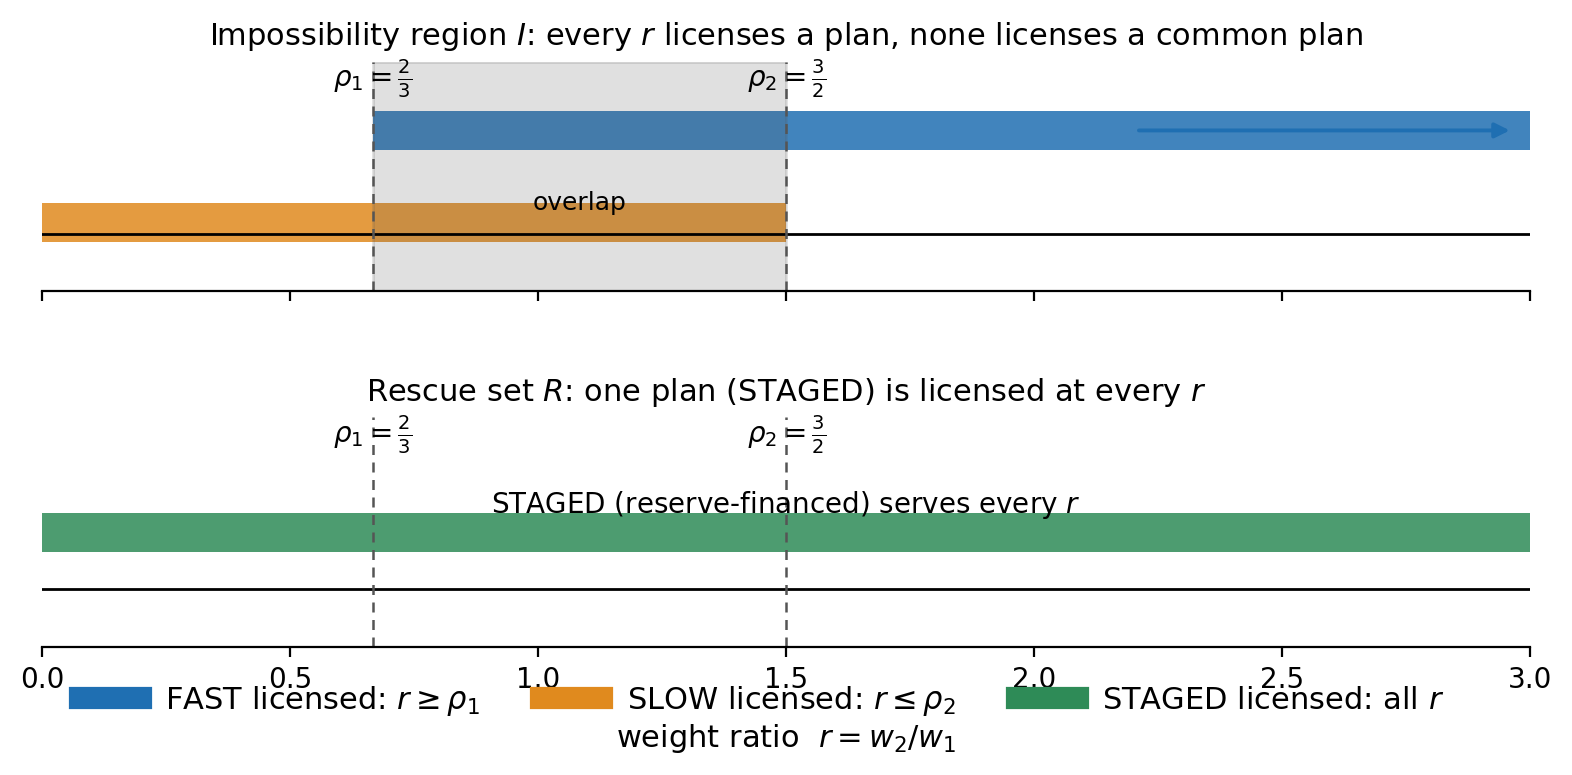
\includegraphics[width=0.9\linewidth]{figS_weight_intervals.png}
\caption{Weight-interval view at the witness point $(x,s_1,s_2)=(\tfrac12,\tfrac65,\tfrac65)$. \act{fast} is licensed exactly for $r\ge\rho_1=\tfrac23$ and \act{slow} exactly for $r\le\rho_2=\tfrac32$. The two intervals together cover every weight ratio $r\ge0$, but neither covers it alone. On the rescue set, \act{staged} supplies the full interval and closes the gap.}
\end{figure}

\section{Verification record}\label{si:verification}

\subsection{Claim layers and evidence}

\begin{table}[!htbp]
\centering\small
\caption{What supports the main classes of claims, and what it does not establish.}
\begin{tabularx}{\textwidth}{@{}>{\raggedright\arraybackslash}p{0.24\textwidth}XX@{}}
\toprule
Claim layer & Evidence & Limitation \\
\midrule
Continuum identities for the witness & Written proofs in the main appendices and SI~S2--S4 & These are paper proofs; they are not established by finite grid checks \\
Finite witness classifications & Exact-integer grid artifact in Figshare v3 (25 checks on a $31^3$ state grid at scale 40) & Verifies only the enumerated rational grid and specified predicates \\
Benchmark arithmetic & 24 exact-rational checks in the SafeTransition v1 artifact & Checks the declared numeric illustration; it does not supply an empirical income model or calibrate a cod stock \\
Selected CES point signs & Four rational logarithm enclosures and a 361-point harmonic identity check reported in the supplementary audit & The scripts/full bounds were not located in the inspected DOI packages; finite samples do not prove a continuum landscape \\
CES continuum statements & Diagonal and pointwise formulas proved in SI~S2--S3 & No global fixed-sum stationary-point, equal-minimum, or slice-closure theorem is claimed in v77 \\
Lean formalization & Pinned source contains selected algebraic witness components and CES rung examples & It does not formalize the full real-exponent nesting, continuity/IVT transfer, or relative-interior argument; no v77 Lean build was run \\
\bottomrule
\end{tabularx}
\end{table}

\subsection{Finite verifiers and their scope}

The Figshare v3 exact-integer verifier enumerates $29{,}791$ states $(x,s_1,s_2)$ on a scale-40 grid and records 25 checks of witness classifications, region identities, licensing thresholds, endpoint comparisons, and hold-prefix persistence. This is exact finite arithmetic on the listed grid, not a proof over the continuum. The SafeTransition v1 benchmark script reports 24 rational checks for the model quantities used in the earlier benchmark package and the abstract action tubes in main-text Table~\ref{main-tab:actions}; v77 changes the unit interpretation and states explicitly that the income coordinate is stipulated, not empirically derived.

The earlier report also listed separate CES, off-diagonal, continuum, and common-shock check counts (57, 50, 44, and 77, respectively). Their scripts and run logs were not present in the two inspected Figshare deposits. A supplementary audit script was rerun with its label-scan input redirected to the current modular SI; that adapted run reproduced four rationally enclosed geometric point verdicts, 361 exact rational harmonic checks, and a numerical tangency search. The geometric verdicts are finite point certificates; the tangency values are high-precision numerical estimates, not certified roots or global extrema. The former 44-check list is not a continuum certificate and is not used to support any global fixed-sum claim in v77. The audit's number of states or checks must not be read as an independent proof of a continuum theorem.

\subsection{Lean coverage and limits}

The cited Lean source is pinned at commit \texttt{6f626ee4\allowbreak 8b2a3a59\allowbreak 282b5df5\allowbreak adda76c8\allowbreak d5993fdc}: \href{https://github.com/MIKEAA2020/general-sustainability/blob/6f626ee48b2a3a59282b5df5adda76c8d5993fdc/lean/Formalizations/P1_AssessmentSeparation.lean}{pinned source file}. Its header explicitly excludes the nesting of real-exponent power means, transfer to non-ladder elasticities, the continuity/IVT step, and relative-interior topology (replaced there by explicit witnesses). The module includes selected algebraic witness identities and rung-specific CES statements, but this does not amount to formalization of the paper's entire pointwise and all-positive-elasticity continuum theorem. The count of declarations is not a coverage metric. No Lean build, dependency-axiom audit, or real-number instantiation check was run for v77; those statuses are not asserted here.

\subsection{Reproduction and version status}

The v77 local package includes assembled and modular TeX, figures, the modified Figure~\ref{main-fig:triangle} source script, a source script for the benchmark-axis unit-label edit, build instructions, hashes, and local QA records. It has no DOI and has not been externally deposited. The existing Figshare and SafeTransition records are version-mismatched; no single inspected deposit reproduces every reported calculation from v77. The main-text Data Availability statement lists those boundaries. The DFO historical anchor was independently traced to Table A2, PDF p.~16, of CSAS SAR 2016/026: $6192.06$ kt over 1983--1989 gives a mean of $884.58$ kt, rounded to $884.6$ kt; the 2015 value is approximately $298.65$ kt. This is a historical assessment-vintage check, not a current threshold update.

\section{Positioning notes, per literature}\label{si:positioning}

\paragraph{Commensurability} The foundation statement that values may be only weakly comparable -- and that this incommensurability is constitutive of ecological economics -- is due to Martinez-Alier, Munda and O'Neill (1998). The main article's operators give one formal model of the distinction that paper draws between strong and weak commensurability.

\paragraph{Maximin and indicator formulations} The characterization of sustainability indicators and the role of maximin and MSY-type reasoning in operationalizing strong-sustainability criteria are developed in Martinet (2011), Cairns and Martinet (2014), and Doyen and Gajardo (2020). This literature includes formal viability and Pareto formulations; the typed operator is one narrow transition-certification idealization and is not presented as a comprehensive or uniquely strongest formalization.

\paragraph{Compensability in multi-criteria decision analysis} Compensability analysis is established in MCDA, including mappings between compensatory aggregation, weak sustainability, and outranking methods (Cinelli, Coles and Kirwan, 2014; Sch\"ar, Pohl and Geldermann, 2025). Weighted-sum limitations on nonconvex Pareto fronts are also well known (Das and Dennis, 1997). The present finite-menu theorem shares convex-hull geometry with these results; it asks a different question about state acceptance and plan selection, and the same quantifier gap can occur for static alternatives.

\paragraph{Acceptance semantics and decision aiding} The protocols of main-text Table~\ref{main-tab:protocols} are decision-aiding constructs: each specifies the rule by which a composite reading sorts a transition into the accepted or rejected category -- the sorting problematic of decision aiding (Roy, 1996; Vincke, 1992). Under the weight-adaptive rule a transition is accepted when every weighting licenses some plan, possibly a different plan for each weighting; the licensing thresholds are then the verdict's weight-sensitivity intervals, analogous to sensitivity analyses applied to composite-indicator rankings (Nardo et al., 2008). The preference-elicitation background is multi-attribute value theory's substitution rates (Keeney and Raiffa, 1976) and the incommensurable-criteria treatment of sustainable development (Munda, 2005).

\paragraph{Viability and robust control} The backward recursion is a typed instance of robust-predecessor, reach--avoid, capture-basin and hybrid-reachability constructions (Aubin, 1991; Aubin, Bayen and Saint-Pierre, 2011; Saint-Pierre, 1994; Lygeros, Tomlin and Sastry, 1999; Aubin and Catt\'e, 2002), with natural-resource management as an established application (De Lara and Doyen, 2008; Doyen et al., 2012). Fractional physical blending and complete-excursion concatenation compare distinct control classes; they are not a mixed/behavioral strategy equivalence. The here-and-now/wait-and-see analogy from adjustable robust optimization concerns the order of plan and weight quantifiers only; the weight is not modeled as a realized disturbance (Ben-Tal et al., 2004).

\paragraph{Planetary boundaries and the safe-and-just space} The typed operator is a formal idealisation of the separate-boundary reading underlying the Planetary Boundaries framework (Rockstr\"om et al., 2009; Steffen et al., 2015), and the same separately-checked-floor logic underlies the safe-and-just-space literature (Raworth, 2012; O'Neill et al., 2018; Fanning et al., 2022). Boundary processes interact and amplify human impacts (Lade et al., 2020), which is why the coupled disturbance regime of S4 is not a remote possibility. The main theorem provides a formal model of \emph{one reason} a noncompensatory stance may be adopted; it does not prove that planetary boundaries ought to be noncompensatory, which is a normative and scientific-design question.

\section{Finite-generation consequence under compact confinement}\label{si:finitegeneration}

This section retains one concise, fully specified consequence of the earlier intergenerational discussion. Let $K$ be a compact state set, and let $V^{(k)}\subseteq K$ be closed, nested decreasing generation constraints with $\bigcap_{k\ge1}V^{(k)}=\varnothing$.

\begin{proposition}[finite-generation obstruction]\label{prop:finitegeneration}
Under these assumptions there is a finite generation $N$ for which $V^{(N)}=\varnothing$. Consequently, no trajectory confined to $K$ can satisfy the requirements through every generation.
\end{proposition}
\begin{proof}
If every $V^{(k)}$ were nonempty, the nested family of closed subsets of compact $K$ would have the finite-intersection property. Compactness would imply $\bigcap_{k\ge1}V^{(k)}\ne\varnothing$, contrary to the hypothesis. Hence some $V^{(N)}$ is empty. Since the sets are decreasing, every later generation set is also empty.
\end{proof}

The common compact confinement is essential to this finite-generation conclusion. Without it, take constant dynamics on $\mathbb R$ and $V^{(k)}=[k,\infty)$. Every finite prefix through generation $N$ is feasible from $x=N$, but no state satisfies all generations. The initial state used for each finite prefix escapes every common compact set.

A separate monotonicity point is not conjectural: for fixed dynamics and a fixed policy class, if safe sets satisfy $K_1\subseteq K_2$, then the viability kernel obeys $\operatorname{Viab}(K_1)\subseteq\operatorname{Viab}(K_2)$. The earlier conjecture that expanding a safe boundary can contract that kernel by admitting a new attractor is therefore withdrawn under those fixed-model assumptions. Any different phenomenon would have to change the dynamics, objective, or policy class as well, and is outside v77.

\section*{References cited in the Supplementary Information}
\begin{itemize}[leftmargin=1.5em,itemsep=1pt]
\item Abaee, A. (2026a). An obstruction calculus for viability under incomplete observation. Zenodo. \url{https://doi.org/10.5281/zenodo.22552616}.
\item Abaee, A. (2026c). Does a surplus-production ladder improve forecasts of Northern cod? A scored test on NAFO 2J3KL. Zenodo. \url{https://doi.org/10.5281/zenodo.22553609}.
\item Abaee, A. (2026d). Verification code and figure pipeline for ``Aggregate indices and transition safety''. Figshare, version 3 (the attached manuscript is Paper1 v42, not this local Paper06 v77 edition). \url{https://doi.org/10.6084/m9.figshare.33764023.v3}.
\item Abaee, A. (2026e). Delay-induced regime change in harvested stocks: the mobilising and protective channels of institutional feedback, and the review interval as control. Zenodo. \url{https://doi.org/10.5281/zenodo.22554217}.
\item Abaee, A. (2026f). \emph{SafeTransition: exact rational certification of transition safety for sustainability assessment}. Software release 1.3.0, Figshare, version 1. \url{https://doi.org/10.6084/m9.figshare.33971389.v1}.
\item Aubin, J.-P. (1991). \emph{Viability Theory}. Birkh\"auser, Boston. Aubin, J.-P., Bayen, A.~M., and Saint-Pierre, P. (2011). \emph{Viability Theory: New Directions}, 2nd ed. Birkh\"auser. Aubin, J.-P., and Catt\'e, F. (2002). \emph{Set-Valued Analysis}, 10(4), 379--416.
\item Ben-Tal, A., Goryashko, A., Guslitzer, E., and Nemirovski, A. (2004). \emph{Mathematical Programming}, 99(2), 351--376.
\item Cairns, R.~D., and Martinet, V. (2014). \emph{European Economic Review}, 69, 4--17.
\item Cardaliaguet, P. (1996). \emph{SIAM Journal on Control and Optimization}, 34(4), 1441--1460.
\item Cinelli, M., Coles, S.~R., and Kirwan, K. (2014). \emph{Ecological Indicators}, 46, 138--148.
\item Das, I., and Dennis, J.~E. (1997). \emph{Structural Optimization}, 14, 63--69.
\item Dearing, J.~A., et al. (2014). Safe and just operating spaces for regional social-ecological systems. \emph{Global Environmental Change}, 28, 227--238.
\item De Lara, M., and Doyen, L. (2008). \emph{Sustainable Management of Natural Resources}. Springer. Doyen, L., et al. (2012). \emph{Ecological Economics}, 75, 32--42. Doyen, L., and Gajardo, P. (2020). \emph{Natural Resource Modeling}, 33(3), e12250.
\item DFO (2016). \emph{Stock Assessment of Northern Cod (NAFO Divs.\ 2J3KL) in 2016}. CSAS Science Advisory Report 2016/026.
\item Fanning, A.~L., O'Neill, D.~W., Hickel, J., and Roux, N. (2022). \emph{Nature Sustainability}, 5(1), 26--36.
\item Keeney, R.~L., and Raiffa, H. (1976). \emph{Decisions with Multiple Objectives}. Wiley.
\item Lade, S.~J., et al. (2020). \emph{Nature Sustainability}, 3(2), 119--128.
\item Lygeros, J., Tomlin, C., and Sastry, S. (1999). \emph{Automatica}, 35(3), 349--370.
\item Martinet, V. (2011). \emph{Journal of Environmental Economics and Management}, 61(2), 183--197.
\item Martinez-Alier, J., Munda, G., and O'Neill, J. (1998). \emph{Ecological Economics}, 26(3), 277--286.
\item Munda, G. (2005). In \emph{Multiple Criteria Decision Analysis: State of the Art Surveys}. Springer, 953--986.
\item Nardo, M., et al. (2008). \emph{Handbook on Constructing Composite Indicators}. OECD.
\item O'Neill, D.~W., Fanning, A.~L., Lamb, W.~F., and Steinberger, J.~K. (2018). \emph{Nature Sustainability}, 1(2), 88--95.
\item Raworth, K. (2012). \emph{Oxfam Policy and Practice: Climate Change and Resilience}, 8(1), 1--26.
\item Rockstr\"om, J., et al. (2009). \emph{Nature}, 461, 472--475. Steffen, W., et al. (2015). Planetary boundaries: Guiding human development on a changing planet. \emph{Science}, 347(6223), 1259855.
\item Roy, B. (1996). \emph{Multicriteria Methodology for Decision Aiding}. Kluwer. Vincke, P. (1992). \emph{Multicriteria Decision-Aid}. Wiley.
\item Saint-Pierre, P. (1994). \emph{Applied Mathematics and Optimization}, 29, 187--209.
\item Schaefer, M.~B. (1954). \emph{Inter-American Tropical Tuna Commission Bulletin}, 1(2), 23--56.
\item Sch\"ar, S., Pohl, E., and Geldermann, J. (2025). \emph{Journal of Multi-Criteria Decision Analysis}, 32, e70013.
\item Sion, M. (1958). \emph{Pacific Journal of Mathematics}, 8(1), 171--176. von Neumann, J. (1928). \emph{Mathematische Annalen}, 100, 295--320.
\end{itemize}

\end{document}
